\documentclass[../main.tex]{subfiles}
\begin{document}
Nella vita di tutti i giorni siamo abituati ad usare un sistema numerico decimale, qui di seguito è riportato un esempio di come funziona invece il sistema numerico binario:
\begin{itemize}
    \item Numeri decimali \begin{align*}
        5374_{10}&=5\cdot 10^3+3  \cdot 10^2+7\cdot 10^1+4\cdot 10^0 \\
        &=5000+300+70+4
    \end{align*}
    \item Numeri binari \begin{align*}
        1101_2&=1 \cdot 2^3+1 \cdot 2^2+0 \cdot2^1+1\cdot2^0 \\
        &=8+4+0+1 \\
        &=13
    \end{align*}
    \item Conversione da decimale a binario \\
    \begin{center}
        $47_{10}$ to binary:
        \begin{align*}
            32\cdot1+16\cdot0+8\cdot1+4\cdot1+2\cdot1+1\cdot1=101111_2
        \end{align*}    
    \end{center}
\end{itemize}

\subsection{Il sistema binario}
Sapendo il numero di bit di un numero binario possiamo determinare:
\begin{itemize}
    \item Il numero di valori che può generare $\rightarrow 2^N$
    \item Il range di numeri possibili da generare $\rightarrow \lbrack0;2^N-1\rbrack$
\end{itemize}
Ad esempio se si hanno a disposizione 3 bit:
\begin{itemize}
    \item $2^3=8$ possibili valori
    \item $\lbrack0;7\rbrack=\lbrack000_2;111_2\rbrack$
\end{itemize}

\subsection{Potenze di due}
È quindi importante essere facilmente in grado di determinare le potenze di due, o almeno una parte di esse:
\begin{figure}[h]
    \centering
    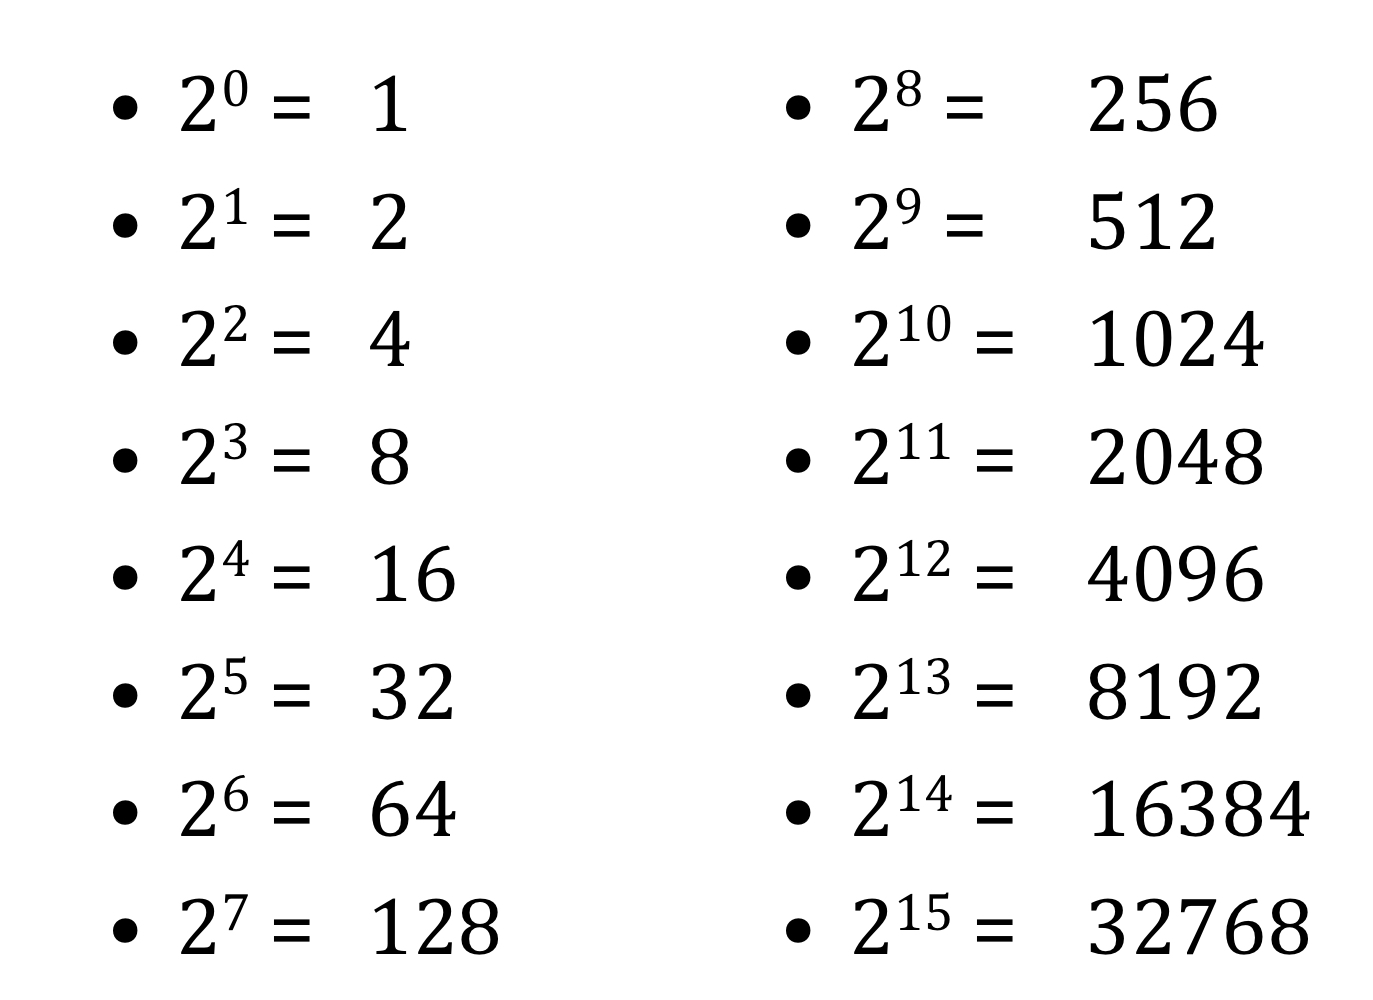
\includegraphics[width=0.4\textwidth]{images/potenzeDiDue.jpeg}
    \caption{Memorizzare fino a $2^9$}
\end{figure}

\pagebreak
\subsection{Sistema esadecimale}
\begin{figure}[h]
    \centering
    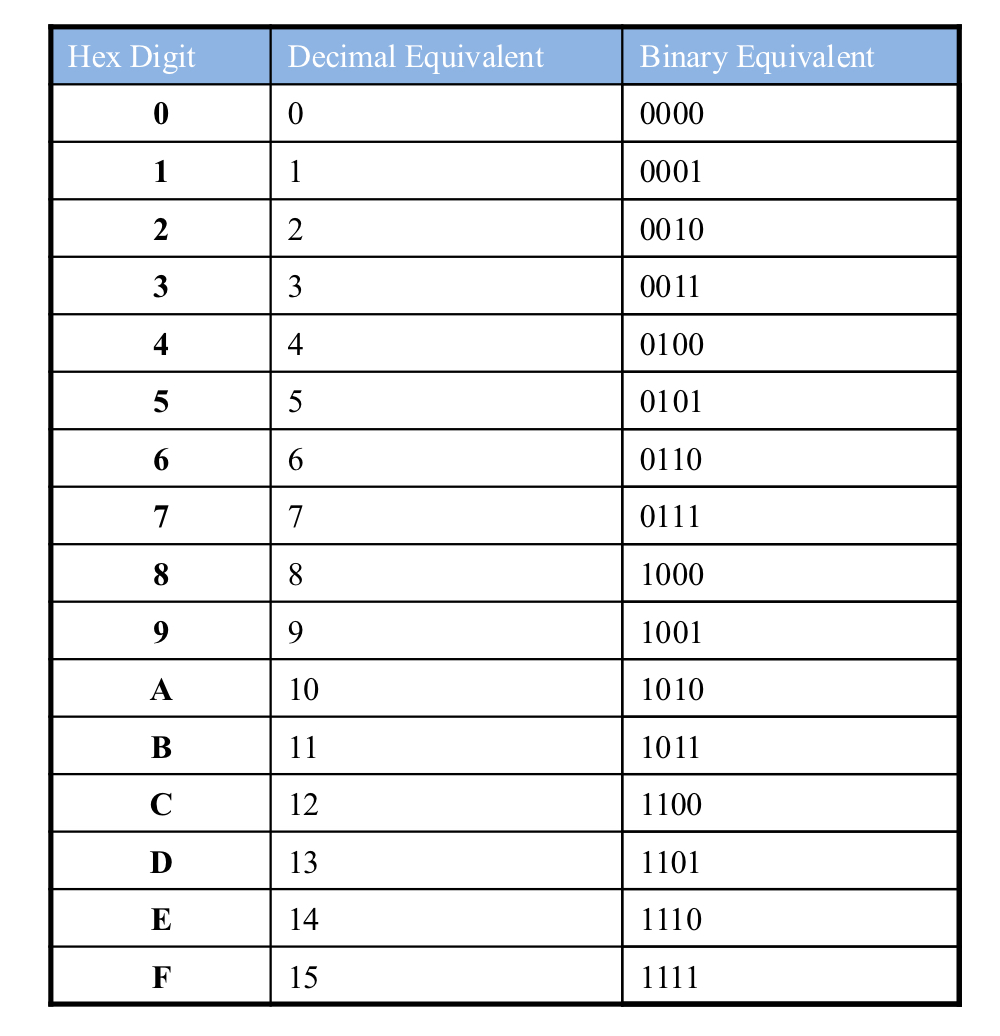
\includegraphics[width=0.5\textwidth]{images/sistemaEsadecimale.jpeg}
    \caption{Numeri esadecimali}
\end{figure}

In questo caso il sistema è simile a quello binario, di seguito sono riportati degli esempi di alcune conversioni:
\begin{itemize}
    \item Da esadecimale a binario: 
        \begin{center}
            $4AF_{16} \rightarrow$ Ogni cifra ha 4 bit

            $0100$ $1010$ $1111_2$
        \end{center}
    \item Da esadecimale a decimale:
    \begin{center}
            $4AF_{16} \rightarrow$ Come per i numeri binari

            $16^2\cdot4+16^1\cdot10+16^0\cdot15=1199_{10}$
        \end{center}
\end{itemize}
\textbf{Nota:} Ogni cifra di un numero esadecimale é composto da un \textbf{nibble}, ovvero 4 bit.
Solitamente con i numeri esadecimali non si parla più di bit più significativo e meno significativo ma di \textbf{byte}.
Un byte sono 8 bit di conseguenza il MSB (Most Significant Byte) saranno le due cifre più a sinistra.

\end{document}